\section{Baseline profiling with Valgrind}
\label{sec:valgrind}
\begin{figure}[!htbp]
  \centering
  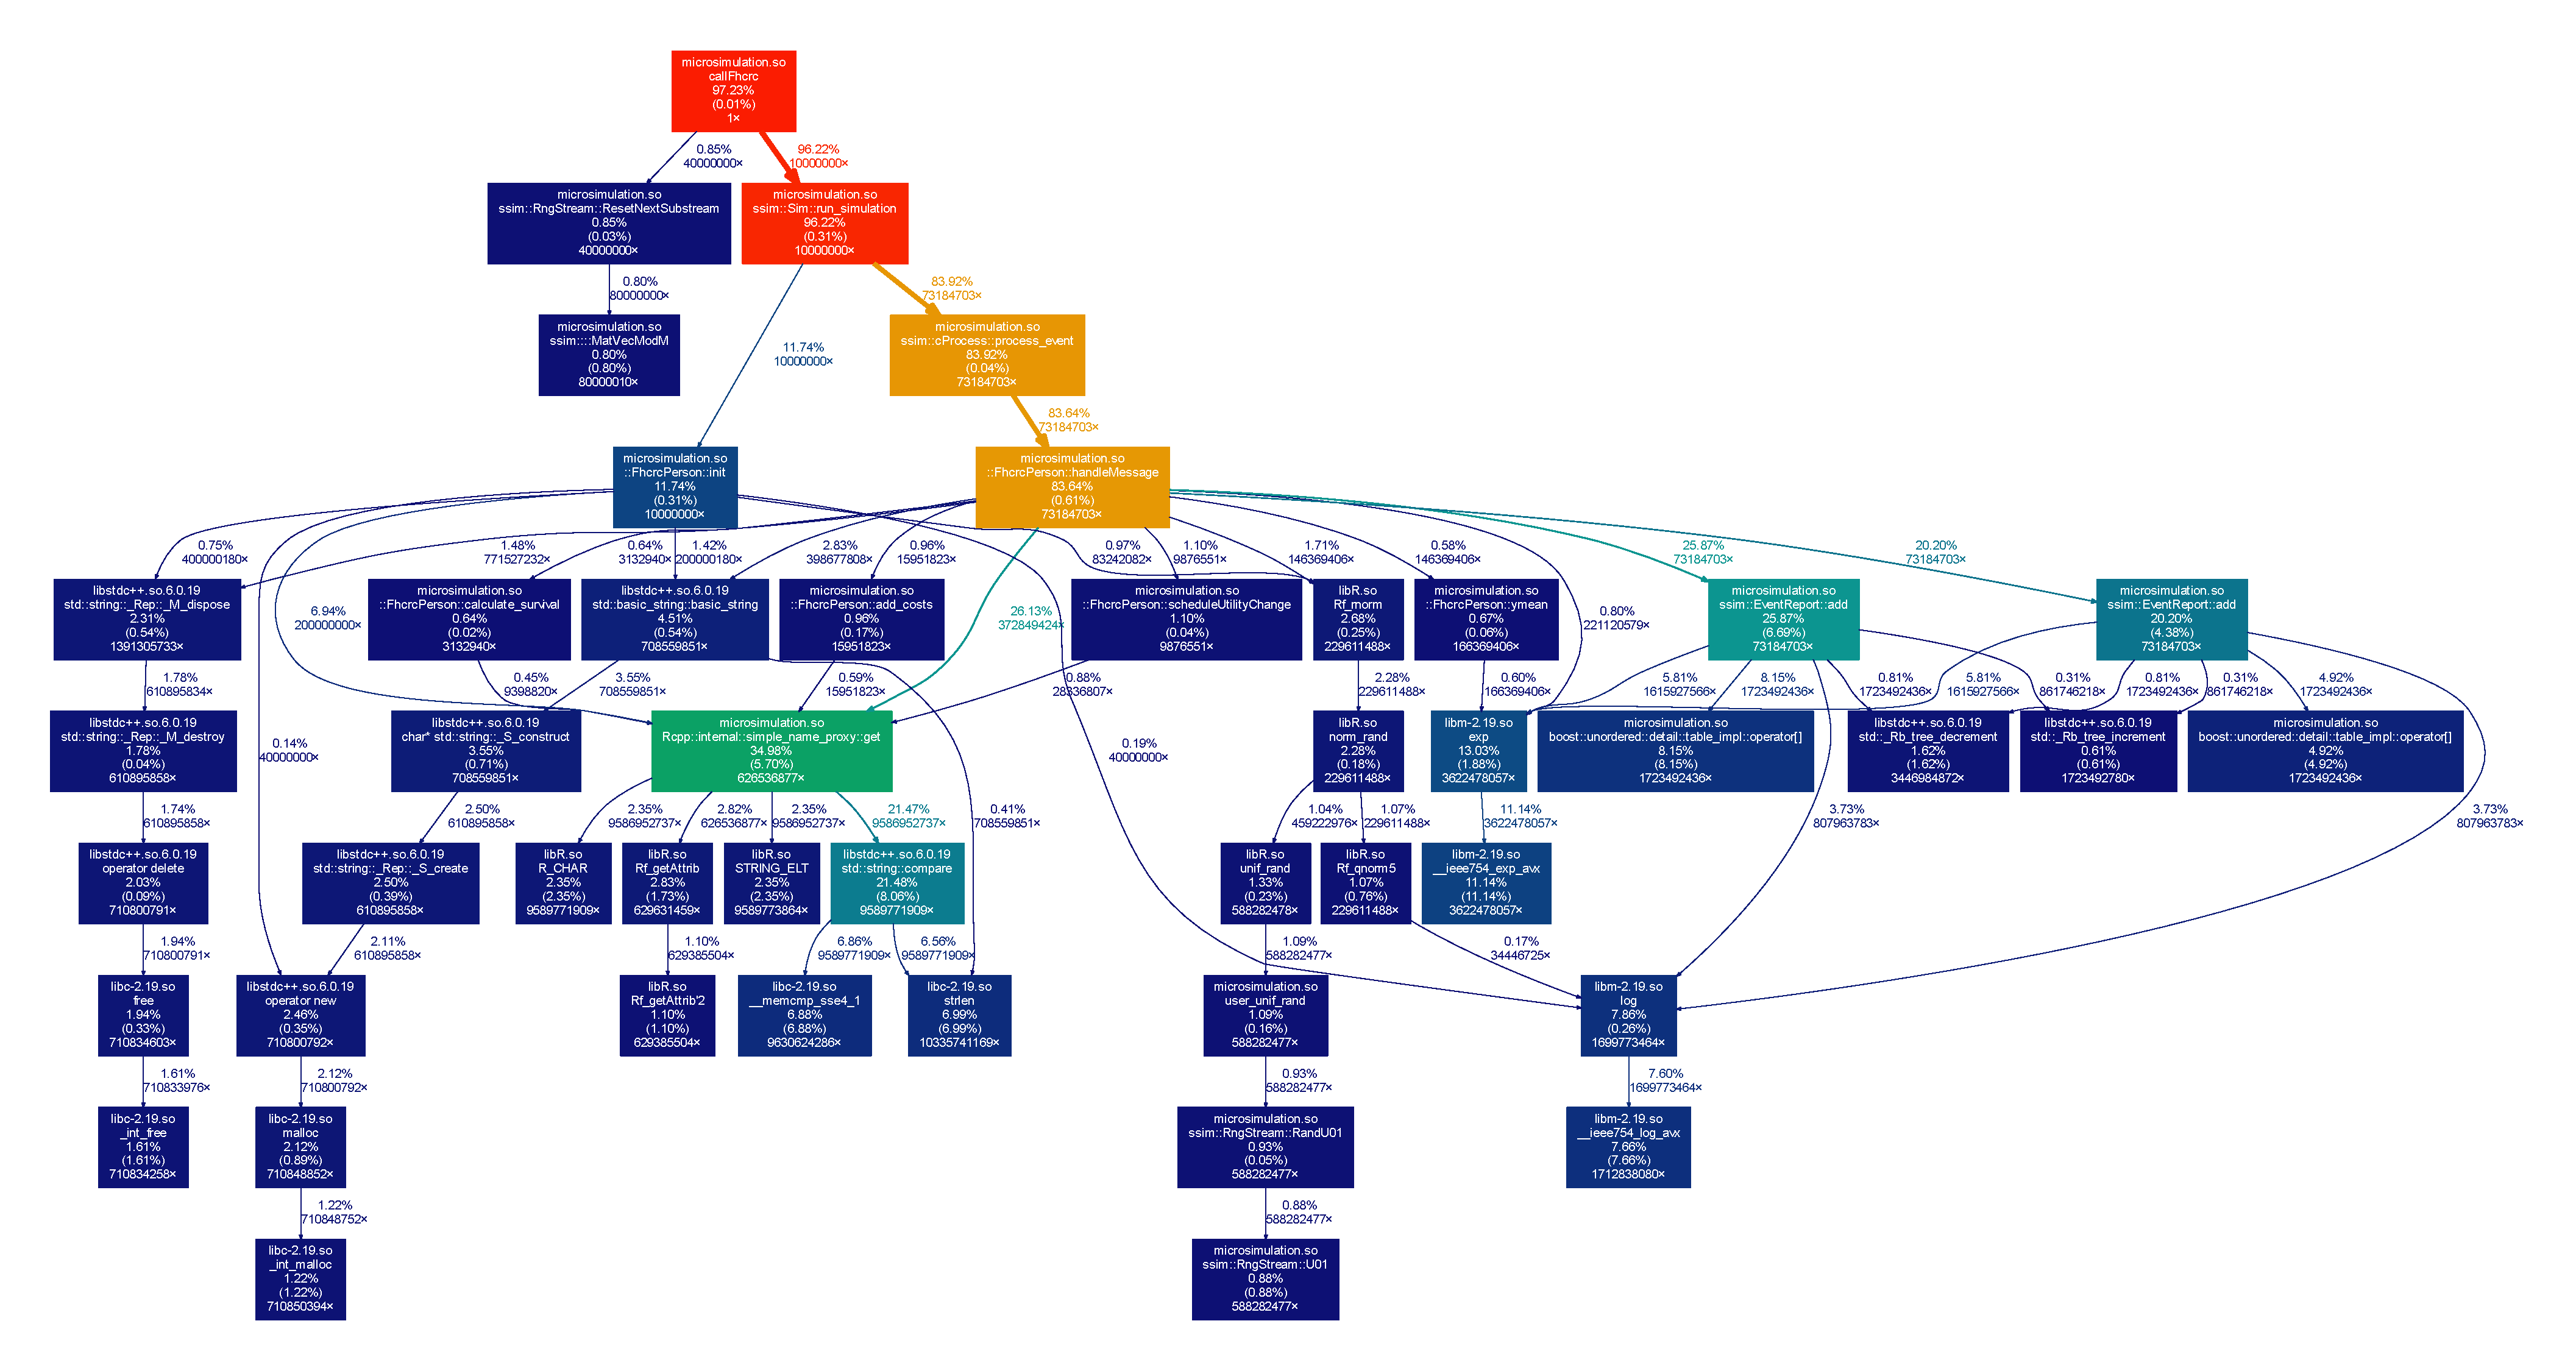
\includegraphics[height=0.45\textheight, angle=90]{images/mediumMotivationalValgrind.pdf}
  \caption{Valgrind measurements at baseline, more extensive then the
    image included in the report.}
  \label{fig:mediumValgrind}
\end{figure}

% \section{Baseline measurements C++}

% \begin{figure}[!htbp]
%   \centering
%   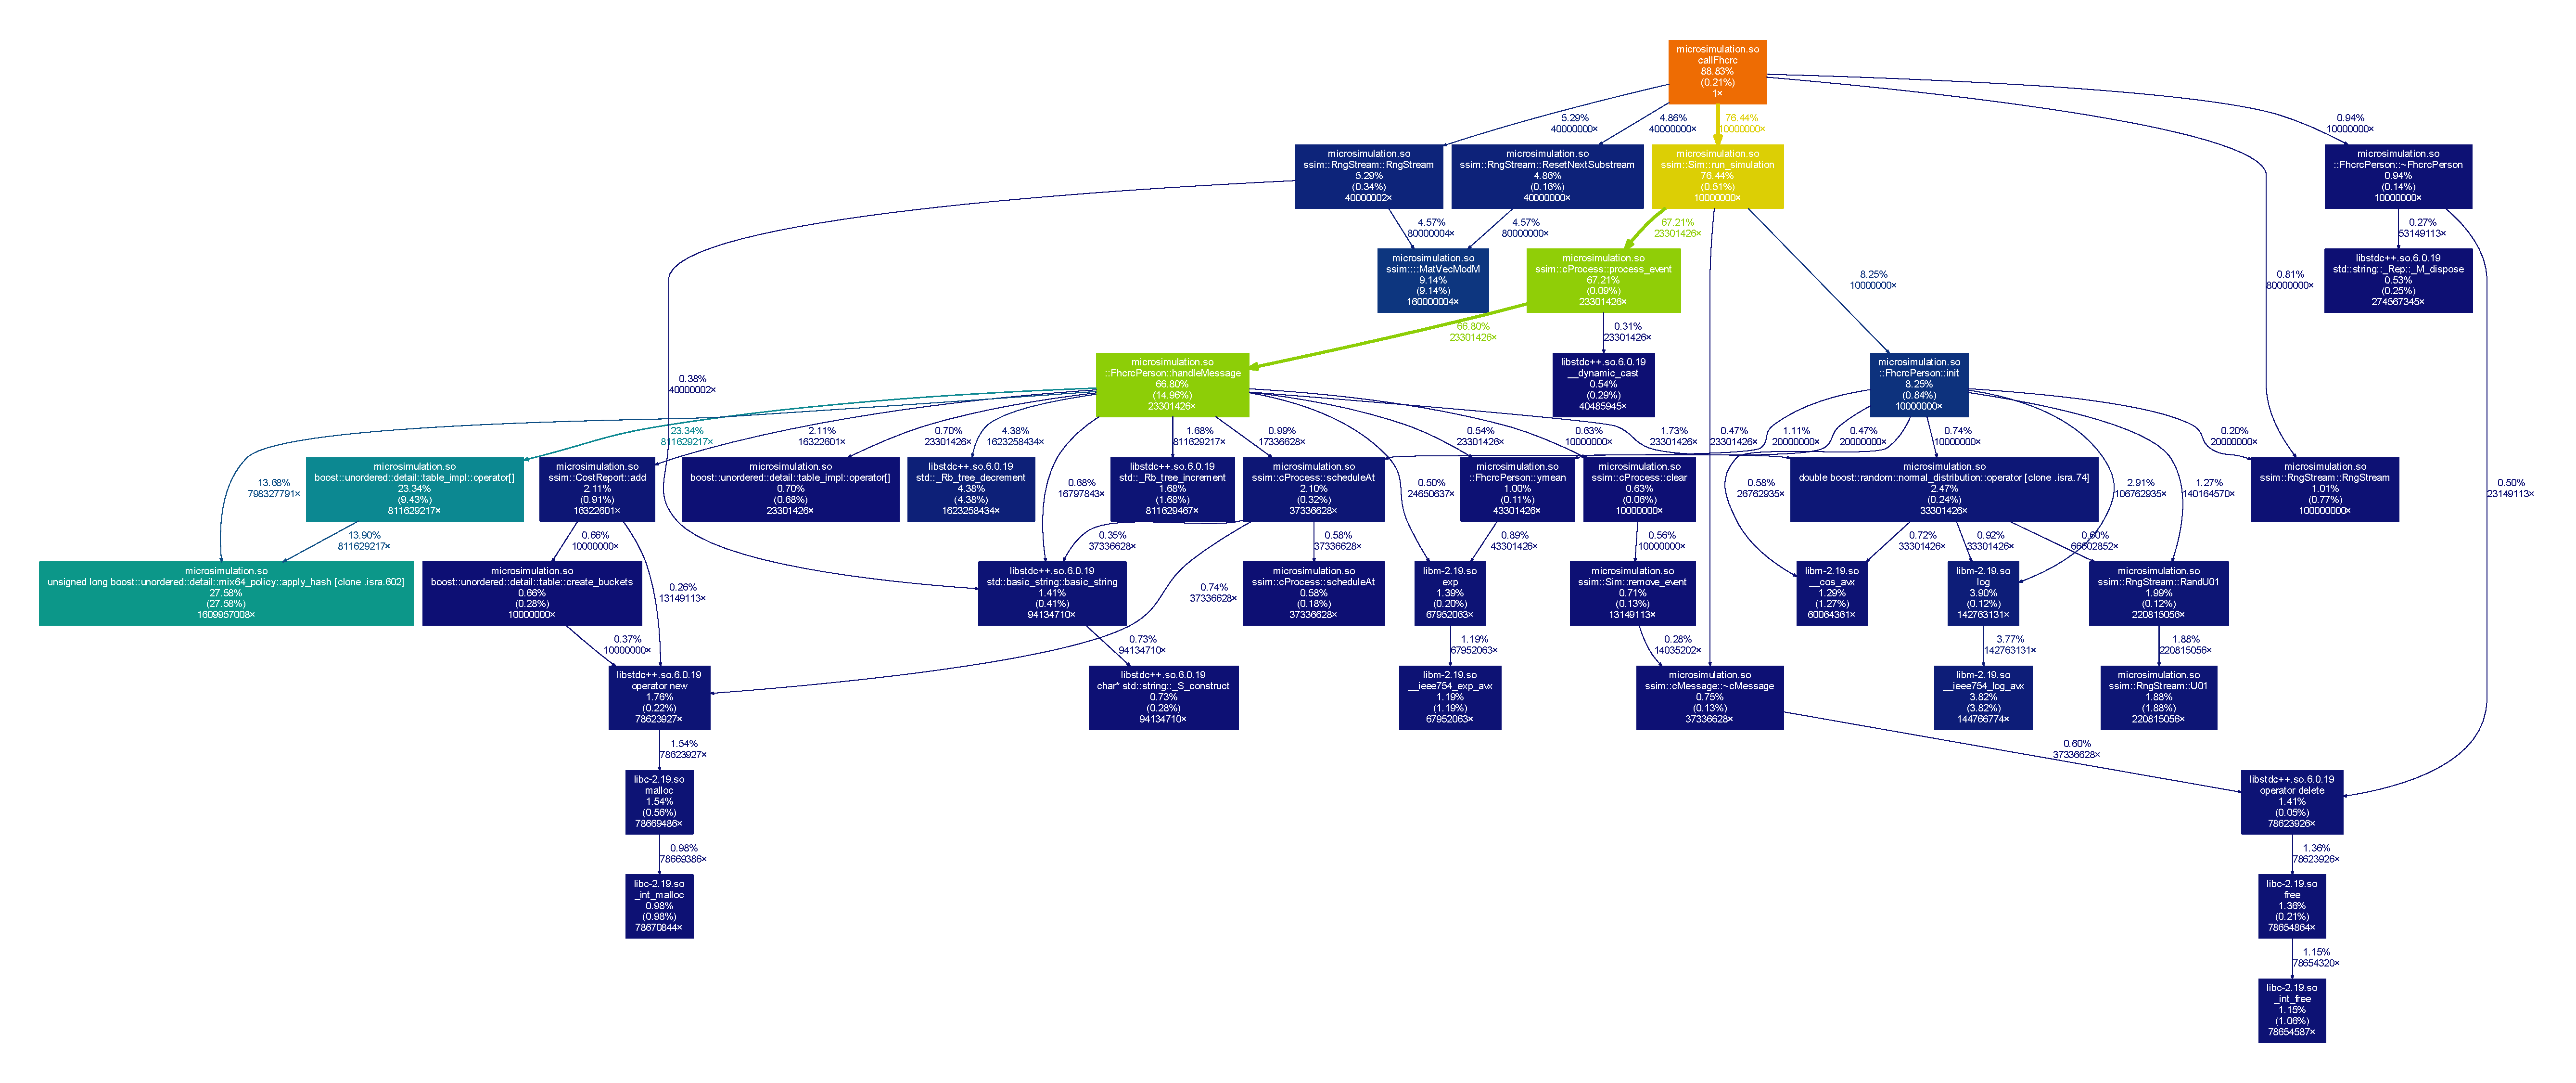
\includegraphics[height=0.50\textheight, angle=90]{images/profBaseLine.pdf}
%   \caption{Valgrind measurements at baseline}
%   \label{fig:baseline}
% \end{figure}


% \section{Simple approach with OpenMP}
% \begin{figure}[!htbp]
%   \centering
%   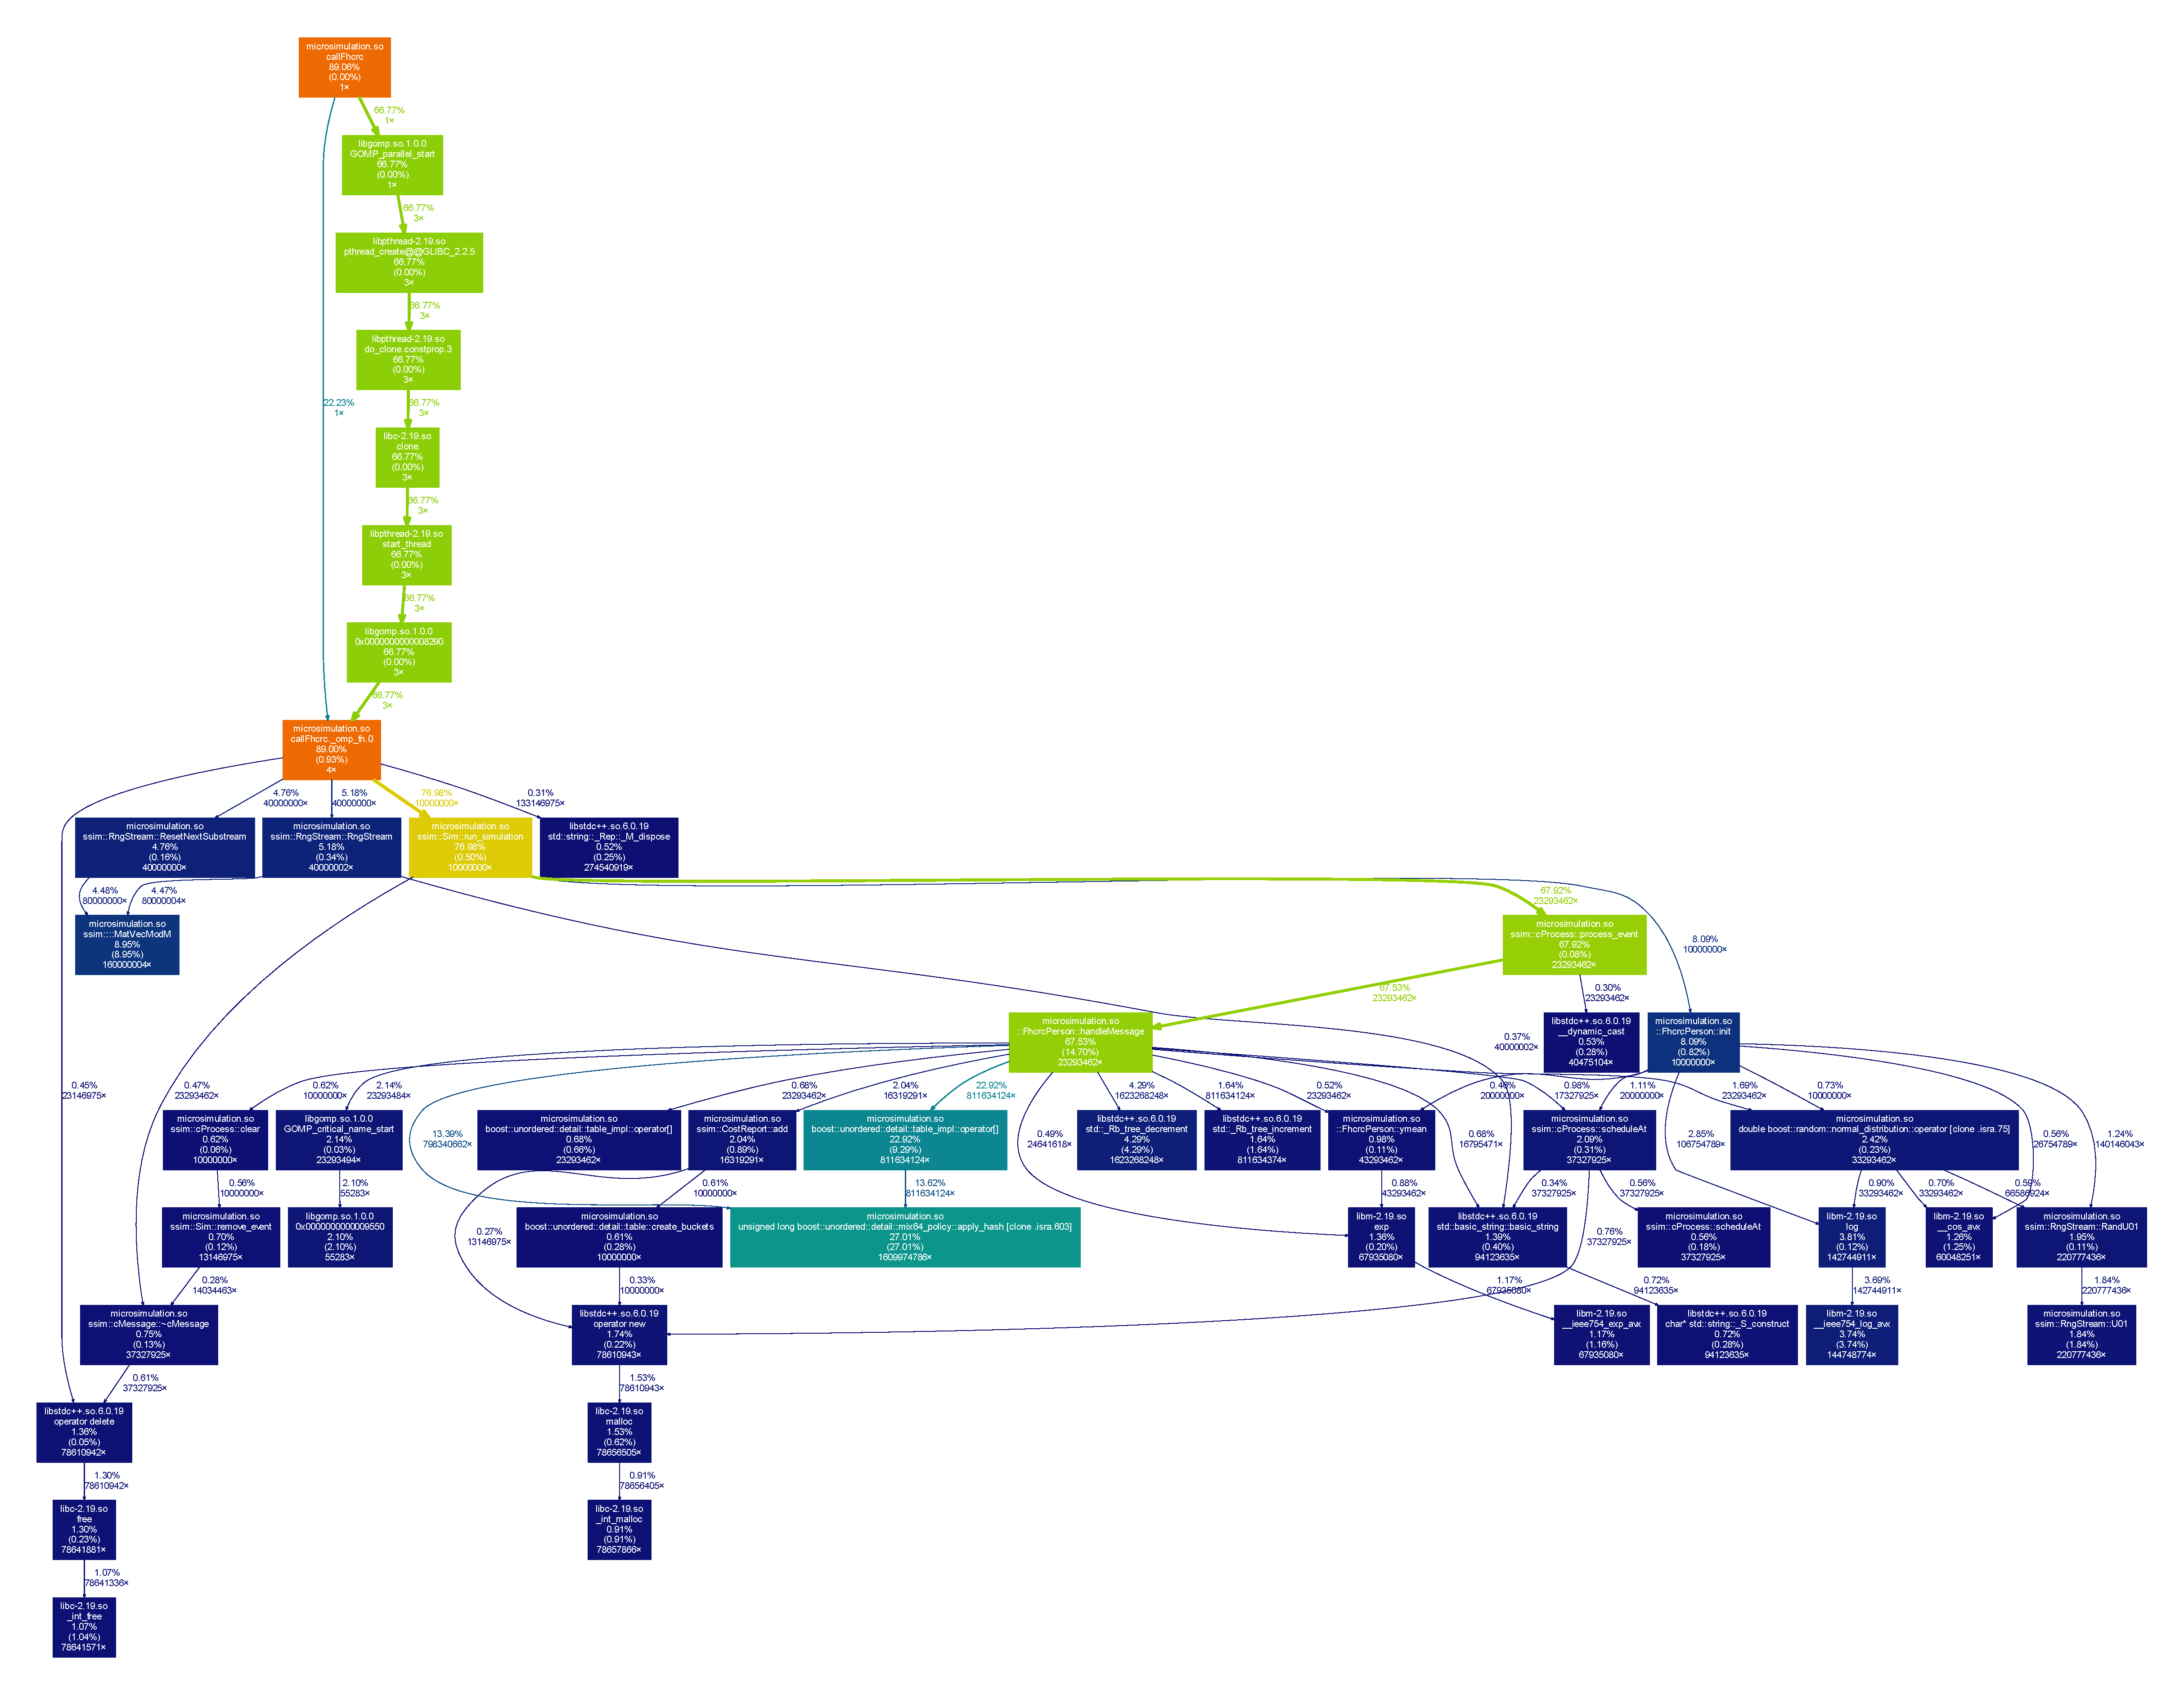
\includegraphics[height=0.85\textheight, angle=90]{images/profOpenMPSimple.pdf}
%   \caption{Valgrind results of the naive openMP implementation}
%   \label{fig:naiveOpenMP}
% \end{figure}

% Here the simulation loop is run in parallel whereas the data output
% and some post-processing is run within a omp critical statement.


%%% Local Variables:
%%% mode: latex
%%% TeX-master: "report"
